\section{Multigrid for finite element methods}
By the definition of convolution \eqref{con1}, we can rewrite \eqref{2d-fe0} and \eqref{2d-fe1} as follows: 
\begin{equation}\label{conA}
A\ast:  \mathbb{R}^{m\times n}\rightarrow \mathbb{R}^{m\times n},~~~A\ast u=f,~~\Leftrightarrow~~ u=\argmin J(v)=\argmin \left(\frac{1}{2}(A\ast v,v)-(f,v)_{l^2}\right)
\end{equation}
where $u=(u_{ij})$, $f=(f_{ij})$, 
\begin{equation}\label{fe0_Ka}
A=\left\{
\begin{array}{ll}
	\begin{pmatrix}
	0 &-1&0\\
	-1& 4&-1\\
	0 &-1& 0
	\end{pmatrix}
&\text{for linear finite element,}	\\
%	\begin{equation}\label{fe1_Ka}
%	K_A=
	\begin{pmatrix}
	-1 &-1&-1\\
	-1& 8&-1\\
	-1 &-1& -1
	\end{pmatrix}
&\text{for bilinear finite element.}
\end{array}\right.
	\end{equation}

It is easy to see that 
$$
\nabla J(v)= A\ast v - f := - r,\quad r=f-A\ast v.
$$
Applying the gradient descent method to \eqref{minProblem}, we obtain the following iterative method: 
\begin{equation}\label{iterativeAst}
u^{k+1} = u^k + \eta r^k,\quad r^k = f-A\ast u^k.
\end{equation}
Here we can clearly see that gradient descent method is equivalent to
damped Jacobi method. Usually, we call this as smoother. 
\begin{lemma}
The gradient descent method \eqref{iterativeAst} for linear finite element converges if $\eta={1\over 8} %\in (0,1/4)
$, and the one for bilinear finite element converges  if $\eta={1\over 16}% \in (0,1/8)
$. Furthermore, the high frequence in $u-u^k$ are damped very rapidly. 
\end{lemma}
\begin{proof}
According to \eqref{iterativeAst} ,
$$
u^{k+1}-u=(I-\eta A)\ast (u^k-u).
$$
The gradient descent method \eqref{iterativeAst} converges if $\rho((I-\eta A)\ast)<1$, namely $\eta\rho(A\ast)<2$. For linear finite element, if $\eta= {1\over 8}$, $\rho(A\ast )<8$, thus the gradient descent method \eqref{iterativeAst} converges.
For bilinear finite element, if $\eta= {1\over 16}$, $\rho(A\ast )<16$, thus the gradient descent method \eqref{iterativeAst} converges.

For linear finite element, let $(\lambda_i, v_i)$ satisfy $A\ast v_i=\lambda_i v_i$ and $0<\lambda_1\leq \lambda_2\leq\cdots\lambda_{N}$ with $N=n^2$. Expand the error $u^k-u$ in terms of eigenvectors $v_i$, namely,
$$
u^k-u=\sum_{i=1}^{N} a_i^kv_i.
$$
Then
$$
u^{k}-u=\sum_{i=1}^{N} a_i^k(1-\eta \lambda_i)v_i=\sum_{i=1}^{N} a_i^0(1-\eta \lambda_i)^{k}v_i.
$$
According to Proposition \ref{prop:A}, it is easy to see that 
$$
1-{1\over 8}\lambda_N\approx {\pi^2\over 4(n+1)^2} \ll 1.
$$
For $\eta={1\over 8}$, the coefficient $a_N^0(1-{1\over 8} \lambda_N)^{k}$ of $v_N$ approximates to zero much faster. This means that high frequency in the error will damp rapidly.
\end{proof}

For an initial guess $u^0$, the left picture in Fig \ref{fig:smooth} plots the error $u-u^0$ and the the right one plots the error $u-u^1$. Fig \ref{fig:smooth} shows that the high frequency in the error of the initial guess $u^0$ is damped after one step of smoothing and results in a smoother error $u-u^1$.
\begin{figure}
\centering
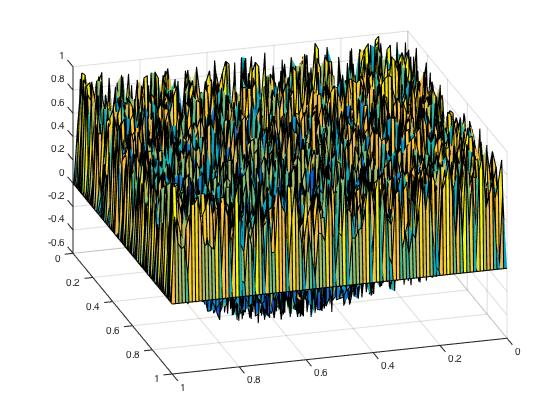
\includegraphics[width=5.5cm,height=5cm]{pictures/smooth0.jpg} \quad
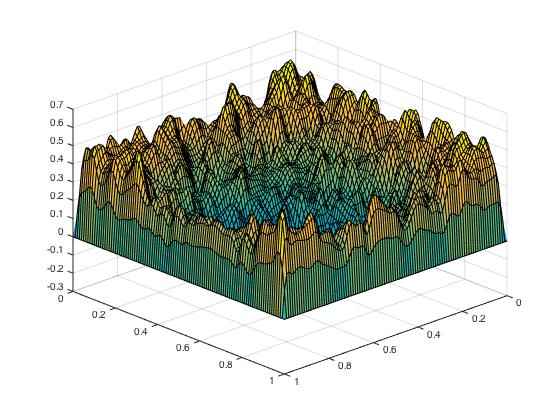
\includegraphics[width=5.5 cm,height=5cm]{pictures/smooth10.jpg}\quad
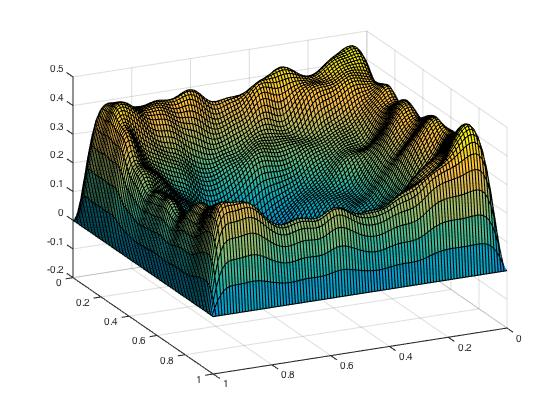
\includegraphics[width=5.5cm,height=5cm]{pictures/smooth50.jpg}\quad
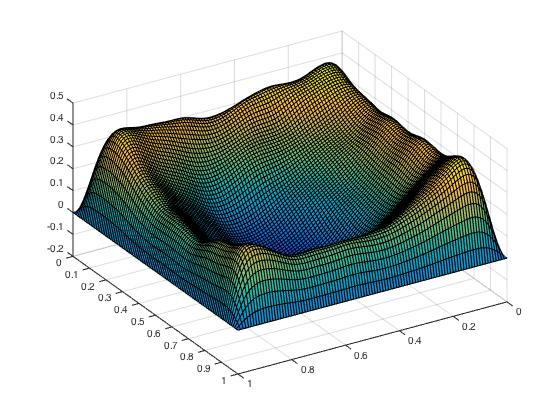
\includegraphics[width=5.5cm,height=5cm]{pictures/smooth100.jpg}
\caption{\footnotesize{The errors of an random initial guess $u^0$, $u^{10}$, $u^{50}$ and  $u^{100}$.}}
\label{fig:smooth}
\end{figure}
%\begin{figure}
%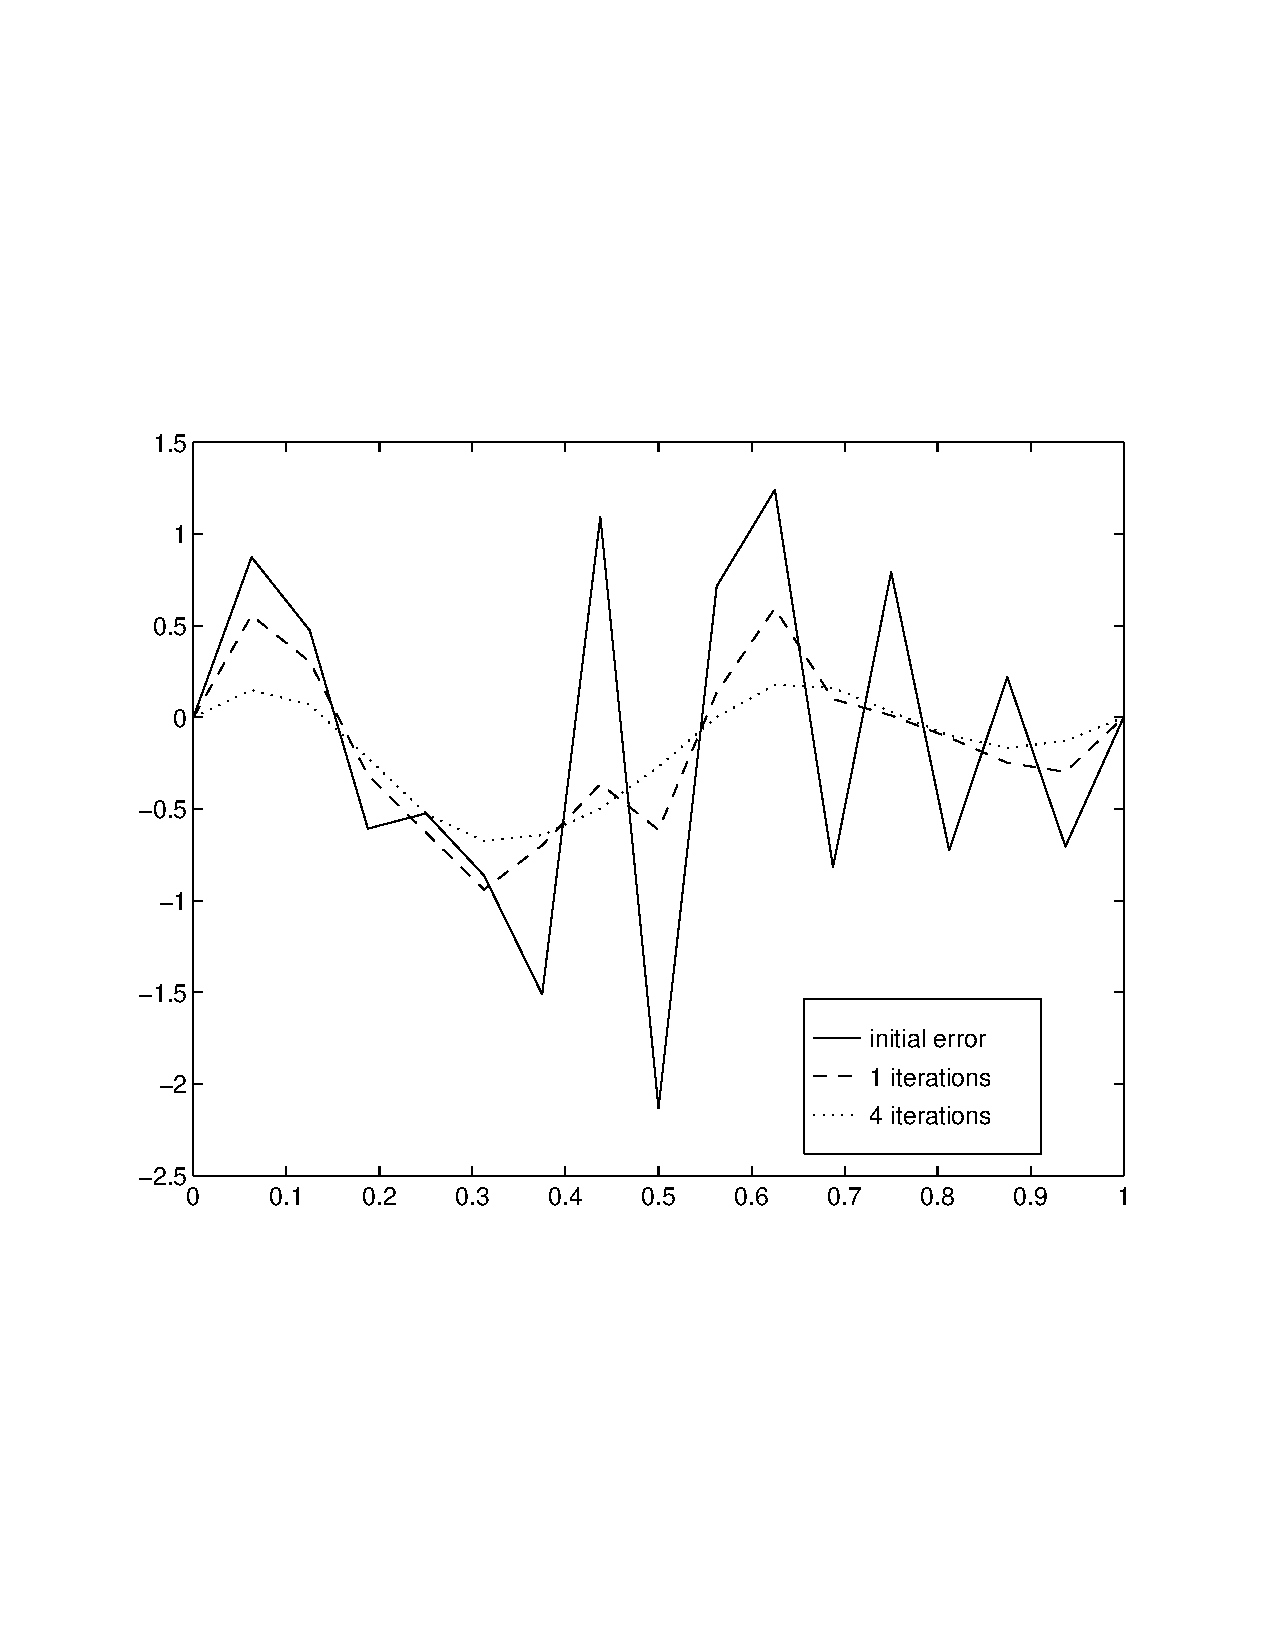
\includegraphics[width=12cm,height=8cm]{pictures/smoothing.pdf}
%\end{figure}
Next, we make the following particular choice:
\begin{equation}
  \label{eta}
\eta={1\over 8}.  
\end{equation}

The gradient descent method can be written in terms of $S_{0}:\mathbb
R^{m\times n}\mapsto \mathbb R^{m\times n}$ satisfying
\begin{equation}
\label{jacobi1}
u^1=(S_{0}f)={1\over 8} f,
\end{equation}
for equation \eqref{2d-fe0} with initial guess zero.
If we apply this method twice, then
$$
u^2=S_1(f) = S_{0} f + S_0(f - A\ast(S_{0}f)),
$$
with element-wise form
\begin{equation} 
\begin{aligned}
u^2_{i,j} &={3\over 16}f_{i,j} + {1\over 64}(f_{i+1,j}+f_{i-1,j}+f_{i,j+1}+f_{i,j-1}).
\end{aligned}
\end{equation}
Then by the definition of convolution \eqref{con1}, we have
 \begin{equation}\label{eq:convS}
u^1= S_{0}\ast f \quad u^2 = S_1 \ast f.
\end{equation}
with
\begin{equation}\label{eq:kernel-S}
S_{0} = {1 \over 8},
\end{equation}
and 
\begin{equation}\label{eq:kernel-S2}
S_1={1\over 64} \begin{pmatrix}
0 & 1 & 0 \\
1 & 12 & 1  \\
0 &1  & 0
\end{pmatrix}.
\end{equation}

Next, we make the following particular choice for the bilinear case:
\begin{equation}
  \label{eta}
\eta={1\over 16}.  
\end{equation}

The gradient descent method can be written in terms of $S_{0}:\mathbb
R^{m\times n}\mapsto \mathbb R^{m\times n}$ satisfying
\begin{equation}
\label{jacobi1}
u^1=(S_{0}f)_{i,j}={1\over 16} f_{i,j},
\end{equation}
for equation \eqref{2d-fe1} with initial guess zero.
If we apply this method twice, then
$$
u^2=S_1(f) = S_{0} f + S_0(f - A\ast(S_{0}f)),
$$
with element-wise form
\begin{equation} 
\begin{aligned}
u^2_{i,j} &={3\over 32}f_{i,j} + {1\over 256}(f_{i+1,j}+f_{i-1,j}+f_{i,j+1}+f_{i,j-1}+f_{i+1,j+1}+f_{i-1,j-1}+f_{i-1,j+1}+f_{i+1,j-1}).
\end{aligned}
\end{equation}
Then by the definition of convolution \eqref{con1}, we have
 \begin{equation}\label{eq:convS}
u^1= S_{0}\ast f \quad u^2 = S_1 \ast f.
\end{equation}
with
\begin{equation}\label{eq:kernel-S}
S_{0} = {1 \over 16},
\end{equation}
and 
\begin{equation}\label{eq:kernel-S2}
S_1={1\over 256} \begin{pmatrix}
1 & 1 & 1 \\
1 & 24 & 1  \\
1 &1  & 1
\end{pmatrix}.
\end{equation}




We note the gradient descent method \eqref{iterativeAst} can be written as
\begin{equation}\label{GD0}
u^k=u^{k-1} + S_0\ast (f-A\ast u^{k-1}).
\end{equation}
\begin{equation}\label{GD1}
u^{2k}=u^{2(k-1)} + S_1\ast (f-A\ast u^{2(k-1)}).
\end{equation}
We can sometimes use $S_1$ and the above identity to define a smoother
directly, namely 
\begin{equation}\label{GD2}
u^{k}=u^{k-1} + S_1\ast (f-A\ast u^{k-1}).
\end{equation}


Similarly, with the smoother obtained by \eqref{eq:convS}, we can define 
$S^{\ell}: \mathbb{R}^{m_\ell \times n_\ell} \mapsto \mathbb{R}^{m_\ell \times n_\ell}$.


First solve the problem on the fine grid $\mathcal T_{\ell}$, denote the solution by $u^{\ell}$, 
\begin{equation}\label{eq:smoothing0}
u^{\ell} \leftarrow u^{\ell} + S^\ell \ast (f^\ell - A_\ell \ast u^{\ell}).
\end{equation}
Denote the error by $e^\ell=u-u^{\ell}$ and the residual
\begin{equation}\label{eq:formresidual}
r^{\ell}=f-A_{\ell}\ast u^{\ell}.
\end{equation}
It is obvious that $A_{\ell}\ast e^\ell=r^{\ell}.$
We need to solve the residual equation
\begin{equation}\label{erreq}
A_{\ell}\ast e^\ell=r^{\ell}.
\end{equation}
The idea of multigrid method is to solve this residual equation on the coarse grid space $\mathcal V_{\ell+1}$ 
and repeat the process until coarsest grid. 

We note that the restriction of \eqref{erreq} to the coarse level $\ell+1$ is
\begin{equation}\label{coarse:correc}
A_{\ell+1}\ast e^{\ell+1}=r^{\ell+1}
\end{equation}
with $r^{\ell+1}=R_\ell^{\ell+1}r^\ell=R\ast r^\ell$.

Denote the finite element approximation to $e_\ell$ on the coarse grid $\mathcal T_{\ell+1}$ by $e_{\ell+1}$. Interpolate the error $e_{\ell+1}$ back to the fine space $\mathcal V_{\ell}$ and add the resulting residual to $u_{\ell+1}$, that is 
\begin{equation}\label{eq:prolongation00}
u^\ell \leftarrow u^{\ell}+P^{\ell}_{\ell+1}e^{\ell+1}
\end{equation}
%as defined in \eqref{mg-prolong} and restriction $R_{\ell}^{\ell+1} = (P_{\ell+1}^{\ell})^T$. 


Now using the smoother $S^\ell$, prolongation $P^{\ell}_{\ell+1}$, restriction $R_{\ell}^{\ell+1}$ and mapping
$A^\ell$ as given in \eqref{eq:def_coarse}, we can formulate the following algorithm
 as a major component of a multigrid algorithm.
\begin{breakablealgorithm}%[!htb]
	\caption{$(u^{1}, u^2, \cdots, u^J) = {\text{MG0}}(f; u^0; J,\nu_1, \cdots, \nu_J)$}
	\label{alg:L-Slash0}
	\begin{algorithmic}
		\State Set up
		$$
		f^1 = f, \quad u^{1}=u^0.
		$$
		\State Smoothing and restriction from fine to coarse level (nested)
		\For{$\ell = 1:J$}
		\For{$i = 1:\nu_\ell$}
		\State
		\begin{equation}\label{eq:smoothing}
		u^{\ell} \leftarrow u^{\ell} + S^\ell \ast (f^\ell - A_\ell \ast u^{\ell}).
		\end{equation}
		\EndFor
		\State Form restricted residual and set initial guess:
		$$
		u^{\ell+1,0} \leftarrow 0, \quad f^{\ell+1} \leftarrow R \ast_2 (f^\ell -  A_\ell \ast u^{\ell}), A_{\ell+1} = R \ast_2 A_\ell \ast (R\ast_2^\top).
		$$
		\EndFor
	\end{algorithmic}
\end{breakablealgorithm}
Here $S^\ell$ can be chosen as $S_0$ or $S_1$ as definition in \eqref{eq:kernel-S} and \eqref{eq:kernel-S2}.

Using the above algorithm, there are different multigrid algorithms such as: $\backslash$-cycle, V-cycle and W-cycle.
Let us now only give one special form of multigrid algorithm for solving \eqref{laplace} as follows.
\begin{breakablealgorithm}%[!htb]
	\caption{$u = {\text{MG1}}(f; u^0; J,\nu_1, \cdots, \nu_J)$}
	\label{alg:L-Slash1}
	\begin{algorithmic}
		\State 
		$$
		u \leftarrow u^0.
		$$
		\State
		$$
		(u^{1}, u^2, \cdots, u^J) = {\text{MG0}}(f; u; J,\nu_1, \cdots, \nu_J).
		$$
		\State Prolongation and restriction from coarse to fine level
		\For{$\ell = J-1:1$}
		\State
		$$
		u^{\ell} \leftarrow u^{\ell} + R  \ast_2^{\top} u^{\ell+1}.
		$$
%		%		\IF{V-cycle}
%		\For{$i = 1:\nu_\ell$}
%		\State
%		$$
%		u^{\ell,i} \leftarrow u^{\ell,i-1} + [B^{\ell,i}]^T (f^\ell - A^{\ell} u^{\ell,i-1})
%		$$
%		\EndFor
%		%		\ENDIF
		\EndFor
		\State
		$$
		u \leftarrow u^{1}.
		$$
	\end{algorithmic}
\end{breakablealgorithm}

If we add the post-smoothing with a symmetric form which means we 
use $[S^\ell \ast ]^\top$ as the smoother, then we can get the V-cycle
version multigrid algorithm.

\begin{breakablealgorithm}%[!htb]
	\caption{$u = {\text{MG2}}(f; u^0; J,\nu_1, \cdots, \nu_J; \nu'_1, \cdots, \nu'_J )$}
	\label{alg:V-cycle}
	\begin{algorithmic}
		\State 
		$$
		(u^{1}, u^2, \cdots, u^J) = {\text{MG0}}(f; u^0; J,\nu_1, \cdots, \nu_J).
		$$
		\State Prolongation and restriction from coarse to fine level
		\For{$\ell = J-1:1$}
		\State
		$$
		u^{\ell} \leftarrow u^{\ell} + R  \ast_2^{\top} u^{\ell+1}.
		$$
		\For{$i = 1:\nu'_\ell$}
		\State
		$$
		u^{\ell} \leftarrow u^{\ell} + S^\ell \ast (f^\ell - A_\ell \ast u^{\ell})
		$$
		\EndFor
				%		\ENDIF
		\EndFor
		\State 
		$$
		u = u^{1}.
		$$
	\end{algorithmic}
\end{breakablealgorithm}
Here $S^\ell $ means the central symmetry of kernel for smoother $S^\ell$ as in the 
definition of \eqref{eq:def_tildeK} in Lemma \ref{lemm:tilde-K}. 

We note that 
$$
\text{MG1}(f; u^0; J,\nu_1, \cdots, \nu_J) = {\text{MG2}}(f; u^0; J,\nu_1, \cdots, \nu_J; 0, \cdots, 0).
$$

Either MG1 or MG2 only represents one cycle in a multigrid process. There many  different ways
to use this basis multigrid cycle. For a given iterate $u$, we need to define a metric to measure the
accuracy of $u$. One way to define it is:
$$
\text{error}(u) = \|f - A\ast u\|  \big/ \|f - A\ast u^0\|.
$$
Sometimes, when we debug a code, we can first try to find the exact solution. $u_{\text{exact}}$, and
then define 
$$
\text{error}(u) = \| u_{\text{exact}} - u\|_A.
$$
Below is one example fo algorithm for application of the basic multigrid cycle, say MG1:
\begin{breakablealgorithm}%[!htb]
	\caption{$u = {\text{multigrid1}}(f; u^0; J,\nu_1, \cdots, \nu_J;  \text{tol})$;}
	\label{alg:multigrid-1}
	\begin{algorithmic}
		\State 
		$$
		u \leftarrow u^0.
		$$
		\While{$\text{error}(u) \ge tol $}
		\State
		$$
		u \leftarrow u + \text{MG1}(f-Au;0;\nu_1, \cdots, \nu_J).
		$$
		\EndWhile
	\end{algorithmic}
\end{breakablealgorithm}

A slightly more general multigrid method. 

\begin{breakablealgorithm}\label{alg:multigrid-Pi}
\begin{enumerate}
\item Initialization of inputs
		$$
		g_1 \leftarrow g, \quad
                u_{1}\leftarrow {\rm random}.
		$$
	\vspace{-.6mm}
\item Smoothing and restriction
  \begin{itemize}
  \item  For $\ell = 1:J$
    \begin{itemize}%3
    \item For $i = 1:\nu_\ell$
		\begin{equation}\label{eq:smoothing}
		u_{\ell} \leftarrow u_{\ell} + S_\ell \ast (g_\ell - A_\ell \ast u_{\ell}).
		\end{equation}
\item  Form restricted residual and set initial guess:
\begin{equation*}
u_{\ell+1,0} \leftarrow\Pi_\ell^{\ell+1}u_{\ell},  \quad g_{\ell+1} \leftarrow R_\ell \ast_2 (g_\ell -  A_\ell \ast u_{\ell}) + A_{\ell+1} \ast u_{\ell+1}^0,
\end{equation*}
    \end{itemize} %3
  \end{itemize}
\item  Prolongation with post-smoothing
  \begin{itemize} %4
  \item For {$\ell = J-1:1$}
		$$
		u_{\ell} \leftarrow u_{\ell} + R_\ell  \ast_2^{\top} (u_{\ell+1}-u_{\ell+1}^0).
		$$
		
                \begin{itemize}
  \item For $i = 1:\nu'_\ell$
		$$
		u_{\ell} \leftarrow u_{\ell} + S_\ell' \ast (g_\ell - A_\ell \ast u_{\ell})
		$$
                \end{itemize}
                \end{itemize} %4
\item Output
		$$
u_1
		$$
\end{enumerate} %1
\end{breakablealgorithm}

\section{Numerical examples}
We consider to solve 
\begin{equation}
\label{laplacenu}
-\Delta u = f,  \mbox{ in } \Omega,\quad
u=0  \mbox{ on } \partial\Omega,\quad
\Omega=(0,1)^2.
\end{equation}
For the $x$ direction and the $y$ direction, we consider the partition:
\begin{equation}\label{partitionyx}
 0=x_0<x_1<\cdots<x_{n+1}=1, \quad x_i=\frac{i}{n+1},\quad (i=0,\cdots,n+1);
 \end{equation}
 \begin{equation}\label{partitiony}
 0=y_0<y_1<\cdots<y_{n+1}=1, \quad y_j=\frac{j}{n+1},\quad (j=0,\cdots,n+1).
\end{equation}
We use linear finite to discretize the 2D Laplacian equation \eqref{laplacenu}.  The size of 
unknowns is $n^2$. We use gradient descent method as smoother in the multigrid method. 
\begin{table}\label{table:multivsGS}%[htdp]
\begin{center}
\begin{tabular}{|c||c|c|}
\hline \hline
Size of Unkowns & Gauss-Seidel for $A$ & Multigrid for $A$ \\ \hline\hline %& V + PCG for $A$\\ \hline %\hline
225  &  226/0.04s     &    13/0.004s \\ \hline %&\onslide<3->{\brown{5/0.003s}}  \\ \hline
961   &  910/0.26s      & 13/0.007s
\\ \hline %& \onslide<5->{\brown{5/0.005s}} \\ \hline 
3969   &  3,044/2.40s   &13/0.021s  \\ \hline %&  \onslide<7->{\brown{5/0.016s}} \\ \hline 
16,129   & 9,869/31.45s    &13/0.08s \\ \hline %& \onslide<9->{\brown{5/0.06s}}  \\ \hline 
65,025   &  30,226/347.38s  &13/0.3s\\ \hline %& \onslide<11->{\brown{5/0.22s}} \\   \hline \hline
\end{tabular}
\caption{Number of iterations for $\| Ax - b \|/ \|b\| \leq 10^{-6}$.}
\end{center}
\end{table}
\vspace{-30pt}
\begin{figure}[!ht]
\centering
%\setlength{\abovecaptionskip}{0pt}
%\setlength{\belowcaptionskip}{0pt}
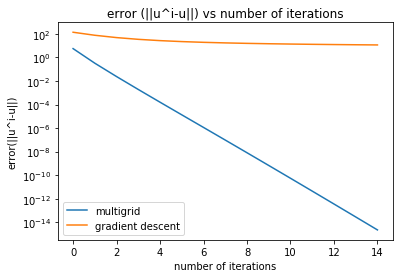
\includegraphics[width=10cm]{figures/mgcompare.png}
\caption{ Comparison GD with Multigrid.}
\label{fig:Hmesh}
\end{figure}

From the Table \ref{table:multivsGS} and Figure \ref{fig:Hmesh}, we can see that the multigrid method is much faster than Gauss-Seidel method and is uniform with respect to the size of unknowns. 






